\newcommand{\exinventory}{
  mail.example.com\\

  [webservers] \\
  foo.example.com \\
  bar.example.com \\
  
  [dbservers] \\
  one.example.com \\
  two.example.com \\
  three.example.com}

\chapter{\ifenglish Background Knowledge and Theory\else ทฤษฎีที่เกี่ยวข้อง\fi}

การทำโครงงาน เริ่มต้นด้วยการศึกษาค้นคว้า ทฤษฎีที่เกี่ยวข้อง หรือ งานวิจัย/โครงงาน ที่เคยมีผู้นำเสนอไว้แล้ว ซึ่งเนื้อหาในบทนี้ก็จะเกี่ยวกับการอธิบายถึงสิ่งที่เกี่ยวข้องกับโครงงาน เพื่อให้ผู้อ่านเข้าใจเนื้อหาในบทถัดๆ ไปได้ง่ายขึ้น

\section{Ansible}
\hspace{0.5in} Ansible คือ Open Source Software ที่ทำหน้าที่เป็นเครื่องมือสำหรับการจัดการระบบ (IT automation) ที่ใช้เพื่อควบคุมและจัดการระบบต่างๆ บนเครือข่าย ใช้งานง่าย มีประสิทธิภาพ และมีความยืดหยุ่นสูง เขียนด้วยภาษา python และใช้ SSH (Secure Shell) ในการเชื่อมต่อกับระบบต่างๆ Ansible ทำงานโดยใช้ Playbook ซึ่งเป็นไฟล์ YAML (Yet Another Markup Language) ที่กำหนดชุดของ tasks ที่จะรันบนระบบปลายทาง \\
รูปที่ \ref{fig:ansible_works} แสดงวิธีการทำงานของ Ansible

\begin{figure}
  \begin{center}
    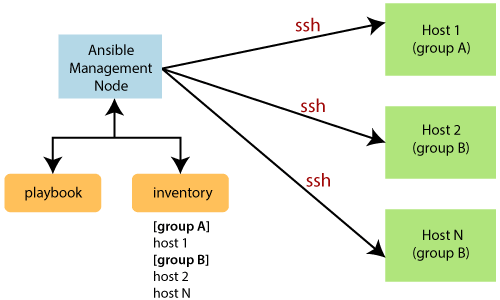
\includegraphics[scale=0.55]{ansible-works.png}
  \end{center}
  \caption[Poem]{วิธีการทำงานของ Ansible}
  \label{fig:ansible_works}
\end{figure}

\subsection{Inventory}
\hspace{0.5in} ไฟล์ที่ระบุรายการระบบปลายทางที่จะจัดการ \\
รูปที่ \ref{fig:inventory.ini} แสดงการเขียนไฟล์ Inventory.ini

\begin{figure}
  \centering
  \fbox{
     \parbox{.6\textwidth}{\exinventory}
  }
  \caption[Sample figure]{การเขียนไฟล์ Inventory.ini}
  \label{fig:inventory.ini}
\end{figure}

\subsection{Playbook}
\hspace{0.5in} ไฟล์ YAML ที่กำหนดชุดของ tasks ที่จะรันบนระบบปลายทาง \\
รูปที่ \ref{fig:ansible_playbook} แสดงการเขียน Playbook

\begin{figure}
  \begin{center}
    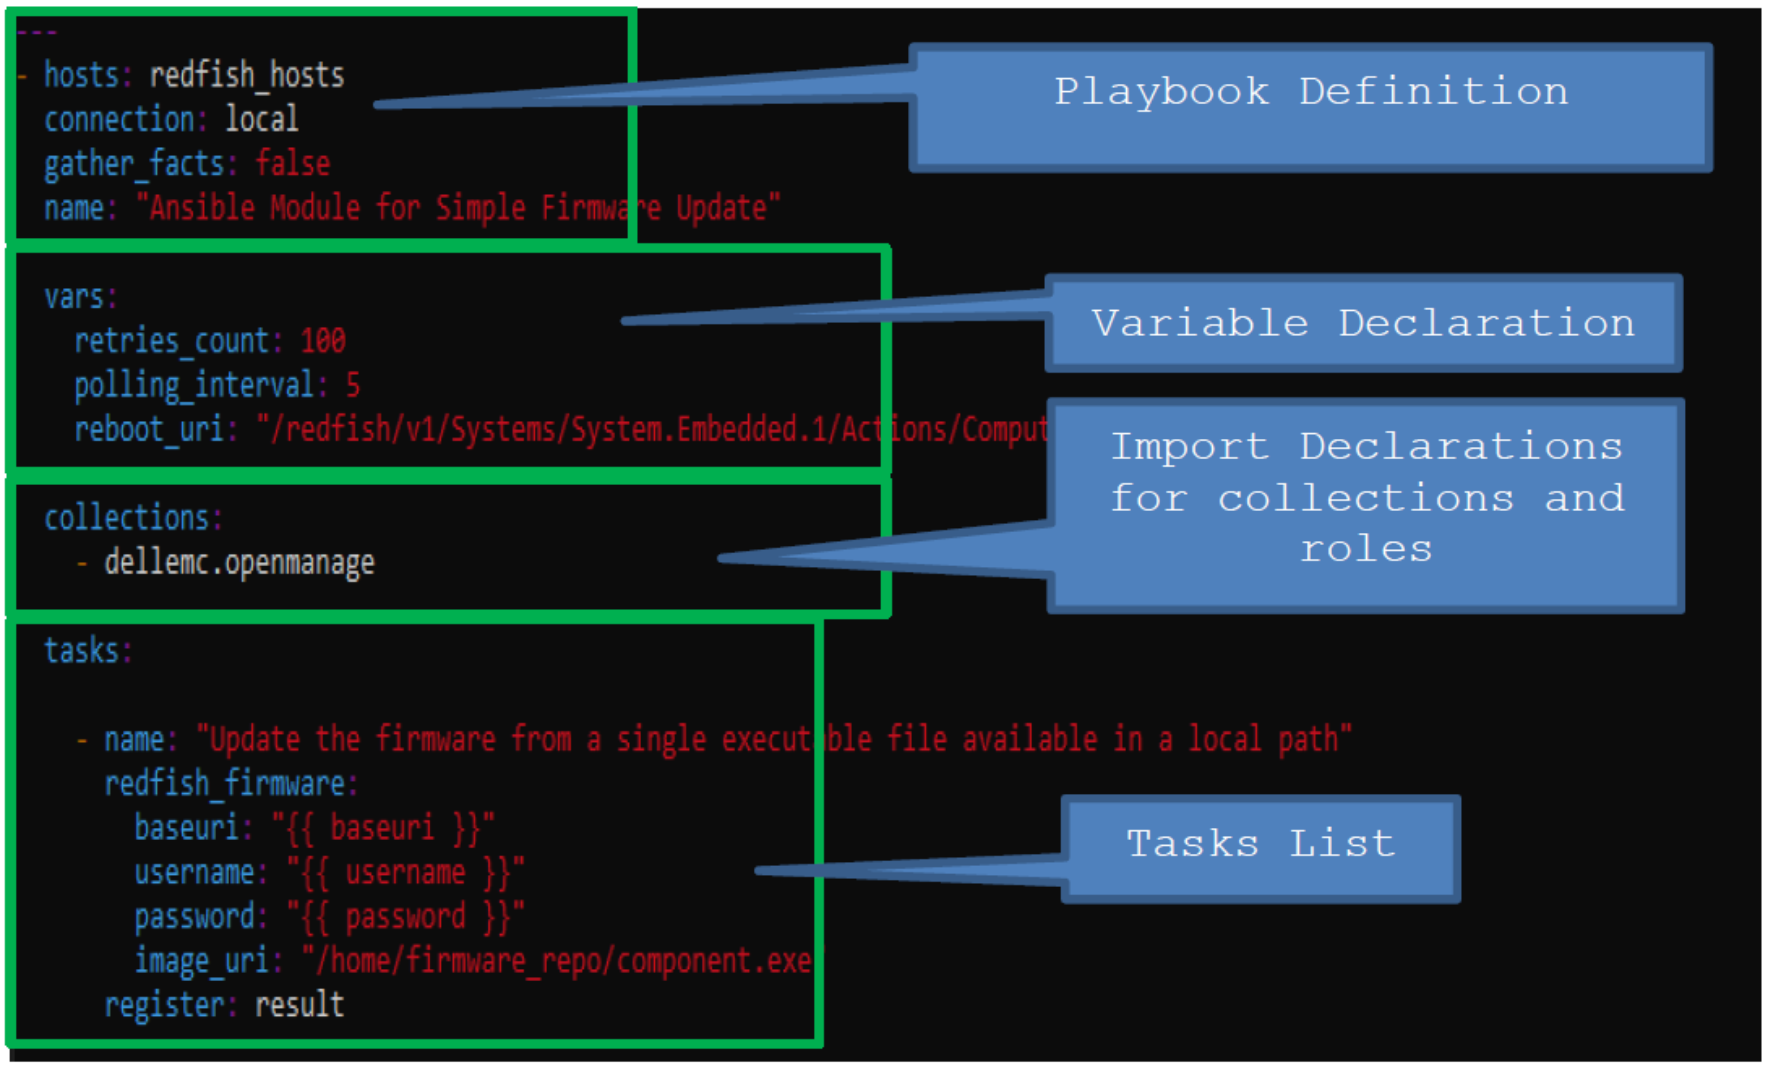
\includegraphics[scale=0.9]{playbook.png}
  \end{center}
  \caption[Poem]{การเขียนไฟล์ playbook}
  \label{fig:ansible_playbook}
\end{figure}

\subsection{Modules}
\hspace{0.5in} โมดูล python ที่ใช้เพื่อดำเนินการจัดการ tasks ต่างๆบนระบบปลายทาง
\subsection{Roles}
\hspace{0.5in} กลุ่มของ tasks ที่สามารถ reuse ได้

\section{AWX}
\hspace{0.5in} AWX เป็นเว็บอินเตอร์เฟสสำหรับ Ansible ช่วยให้ผู้ใช้สามารถจัดการ Ansible playbooks และ inventories ผ่านเว็บเบราว์เซอร์โดยไม่ต้องพึ่ง command line ทำให้การจัดการโครงสร้างพื้นฐาน IT ด้วย Ansible นั้นง่ายขึ้นและสะดวกยิ่งขึ้น

\begin{figure}[h]
  \begin{center}
    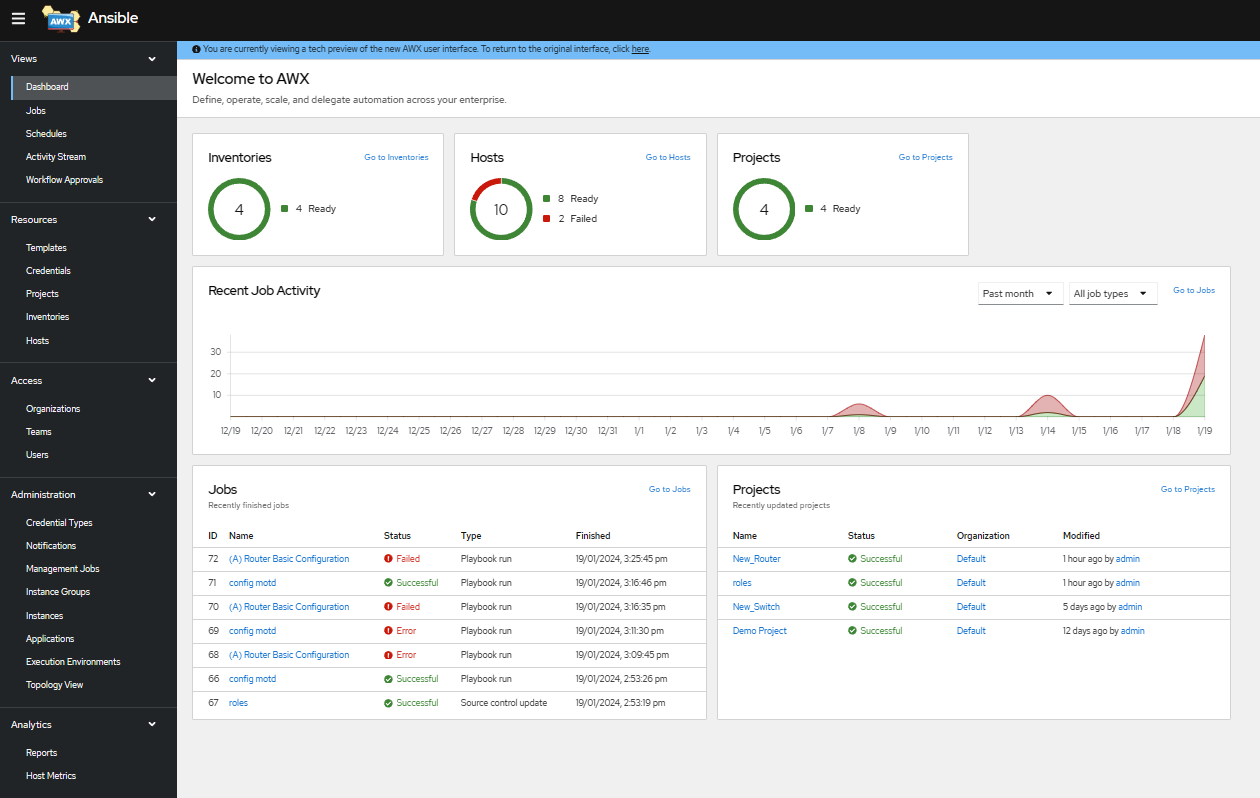
\includegraphics[scale=0.55]{awx.png}
  \end{center}
  \caption[Poem]{ตัวอย่างการแสดงผลของ AWX}
  \label{fig:ansible_playbook}
\end{figure}

\hspace{0.3in} โดยส่วนสำคัญของ AWX ได้แก่


\subsection{Dashboard}
\hspace{0.5in} แสดงสถานะทั้งหมดของ AWX และการทำงานของ ansible เอาไว้โดยรวม เช่น จำนวน hosts จำนวน project หรือสถานะของงานที่เคยเรียกใช้ ว่าสำเร็จหรือไม่สำเร็จ

\subsection{Inventory}
\hspace{0.5in} ใช้สำหรับจัดกลุ่มเพื่อรวบรวม และจัดการ hosts ต่างๆ ที่จะต้องใช้งานเอาไว้ โดยสามารถเพิ่มหรือจัดการ hosts เหล่านั้นเองได้

\subsection{Projects}
\hspace{0.5in} ใช้จัดการโค้ดของ ansible ที่จะใช้งาน ซึ่งคล้ายกับ git โดยจะเก็บ playbook เก็บ inventory และตัวแปรต่างๆที่เกี่ยวข้องเอาไว้

\subsection{Hosts}
\hspace{0.5in} แสดงรายการ host ต่างๆที่เอาไว้ใช้งาน โดย hosts เหล่านี้จะถูกจัดเก็บอยู่ใน inventory ซึ่งจะแสดงว่า host แต่ละตัวนั้นถูกเก็บโดย inventory ไหนบ้าง

\subsection{Credentials}
\hspace{0.5in} ใช้สำหรับยืนยันตัวตนเช่น ชื่อผู้ใช้ รหัสผ่าน คีย์ ssh หรือข้อมูลอื่นๆที่ ansible ต้องการ

\subsection{Templates}
\hspace{0.5in} ใช้สร้างงานต่างๆ โดยจะทำงานร่วมกับ playbook และ inventory ที่เราสร้างไว้ ซึ่งเราสามารถรวม งานหลายๆงานให้ทำงานต่อเนื่องกันไว้ใน template เดียว ผ่าน workflow template

\subsection{Jobs}
\hspace{0.5in} แสดงผลลัพธ์และสถานะของงานนั้นๆที่เคยถูกเรียกใช้ทั้งหมด ว่าสำเร็จหรือไม่สำเร็จ หรือมี error เกิดขึ้น

\section{\ifenglish%
\ifcpe CPE \else ISNE \fi knowledge used, applied, or integrated in this project
\else%
ความรู้ตามหลักสูตรซึ่งถูกนำมาใช้หรือบูรณาการในโครงงาน
\fi
}
\begin{enumerate}
\item การเข้าใช้เครือข่าย การจัดการระบบเครือข่ายและความรู้ด้านเครือข่ายจากวิชา เครือข่ายคอมพิวเตอร์ (Computer Network 261335) 
\item ชุดคำสั่งการตั้งค่าของระบบเครือข่าย การดูแลระบบเน็ตเวิร์คและการตรวจสอบชุดคำสั่งทางด้านเครือข่ายจากวิชา ปฏิบัติการเครือข่ายคอมพิวเตอร์ (Computer Network Laboratory 261336)
\item กระบวนการพัฒนาโปรแกรมจากวิชาวิศวกรรมซอฟต์แวร์ (Software Engineer 261361)
\end{enumerate}

\section{\ifenglish%
Extracurricular knowledge used, applied, or integrated in this project
\else%
ความรู้นอกหลักสูตรซึ่งถูกนำมาใช้หรือบูรณาการในโครงงาน
\fi
}

\begin{enumerate}
  \item การทำงานของ Ansible
  \item การทำงานและวิธีใช้งาน Ansible AWX
\end{enumerate}
